%%
%% Template intro.tex
%%

\chapter{Background}
\label{cha:back}

In this chapter, we define the social network Facebook central to this study, the source of our data set, notation used throughout 
this thesis, our choice of classification algorithms and finally our testing approach and methodology.

\section{Facebook}
\label{sec:data}

Facebook is the largest and most active social media service in the world (as of September 2012 it had more than 1 billion active users \cite{fbsize}).
Facebook users can create a profile containing personal \emph{preferences} and information including their favourite music, favourite movies, 
inspirational people, interests, age, birthday, etc and have friendships and \emph{interactions} between other users. 

The four main interactions between users are posts (posting something on a friends' wall), 
tags (being mentioned in a friends post or comment), comments (written data on a post) and likes (clicking a like button if a user 
likes a post or comment). The mediums for these interactions are across links (some URL), posts (some Facebook post), 
photos (some uploaded Facebook photo) and videos (some uploaded Facebook video).

Given the enormous scope of \emph{interaction} and \emph{preference} information available for each user, NICTA have developed an application (app) capable of tracking 
and recording all pertinent user information. This app will be discussed in the following section.

%\cite{backstrom2011center} studied two types of user uses of Facebook, explicit communication interaction and viewing attention. Communication 
%is focused on a limited subset of friends whilst viewing attention is dispersed among a much larger set. This supports the approach of testing
%a wide array of user interactiuons and preferences, as each users preferences are driven by where their attention is focused.

\section{Data Set}
\label{sec:linkr}

One issue present in the Facebook paradigm is deciphering whether a user does not like an item, a users Facebook feed (current visible 
personalised Facebook information) is comprised of recent
activity  between their friends, groups, pages, etc giving an enormous scope for potential feed items.
Given the high rate of posting, these top feed items are only displayed for a short period of time. Coupled 
with the fact that Facebook allows users to explicitly like an item, but not dislike it - distinguishing between what 
a user does and does not like becomes difficult.

%While many Facebook users have a friend count which is close to the human real word limit, known as the Dunbar number 
%~\cite{hill2003social}, the \emph{Edge-Rank} algorithm ensures user interactions are focused on a much smaller subset of their friends.

Given this fact, a Facebook app named \emph{LinkR}\footnote{The main developer of the LinkR Facebook App is Khoi-Nguyen Tran, a PhD student at the Australian National University.} was developed \cite{www}.
This app collected information about users, their interactions and preferences as well as a subset of available information about 
their friends. Additionally, the app proposed links to users and asked them to explicitly rate each link as either a like or dislike. 
The app tracked and stored this information for over 100 app users and their 39,000 friends over a 4-month time period. Which is a sufficiently large data-set for 
performing our analysis.

The table below summarises the interactions data collected from both app users and their friends used during subsequent analysis.

\begin{table}[h!]
\centering
	\begin{tabular}{|l|r|r|r|r|} % cols: (left, center, right)
		\hline
		\textbf{App Users} & \textbf{Posts} & \textbf{Tags} & \textbf{Comments} & \textbf{Likes}  \\ \hline
		\textbf{Wall} & 36,539 & 7,711 & 18,266 & 15,999 \\ \hline
		\textbf{Link} & 5,304 & - & 5,757 & 6,566 \\ \hline
		\textbf{Photo} & 4,933 & 28,341 & 8,677 & 8,612 \\ \hline
		\textbf{Video} & 245 & 2,525 & 1,687 & 843 \\ \hline
		 \hline
		\textbf{App Users and Friends} & \textbf{Posts} & \textbf{Tags} & \textbf{Comments} & \textbf{Likes}  \\ \hline
		\textbf{Wall} & 4,301,306 & 1,215,382 & 3,122,019 & 1,887,497 \\ \hline
		\textbf{Link} & 678,612 & - & 693,930 & 995,214 \\ \hline
		\textbf{Photo} & 1,268,816 & 9,620,708 & 3,431,321 & 2,469,859 \\ \hline
		\textbf{Video} & 59,244 & 904,604 & 486,677 & 332,619 \\ \hline
	\end{tabular}
	\caption{Data records for interactions between users. Rows are the type of interaction, columns are the medium of interaction.}
	\label{tab:revpol}
\end{table}

\section{Notation}
\label{sec:notation}

The mathematical notation utilised during this thesis is outlined below.

\begin{itemize}
\item A set of users $U$ of size $N$ each with an associated $I$-element user feature vector $X$ where $X \in \mathbb{R}^I$ (alternatively if a second user is needed $Z \in \mathbb{R}^I$) 
where the length and components of $I$ are uniquely defined for each affinity feature, under their appropriate sections.
\item A set of items $V$.
\item A friend function $Friend_{u,z}$ which is $True$ when users $u$ and $z$ are friends.
\item A liked function $Likes_{u,v}$ which is $True$ when user $u$ likes item $v$.
\item A relationship between user $u$ over some feature index $i$ where this $Relationship_{u,i}$ is uniquely defined under each affinity features section.
\item An alters set for each user $u$ item $v$ pair over some feature index $i$, based on some relationship between other users $z$ and where each of $u$ and $z$ have liked item $v$. 
Where $alters_{u,v,i} = \{z | Relationship_{u,i} \wedge Likes_{u,v} \wedge Likes_{z,v}\}$.

This alters set can be visualised in the figure below:

\begin{figure}[h!]
	\begin{center}
		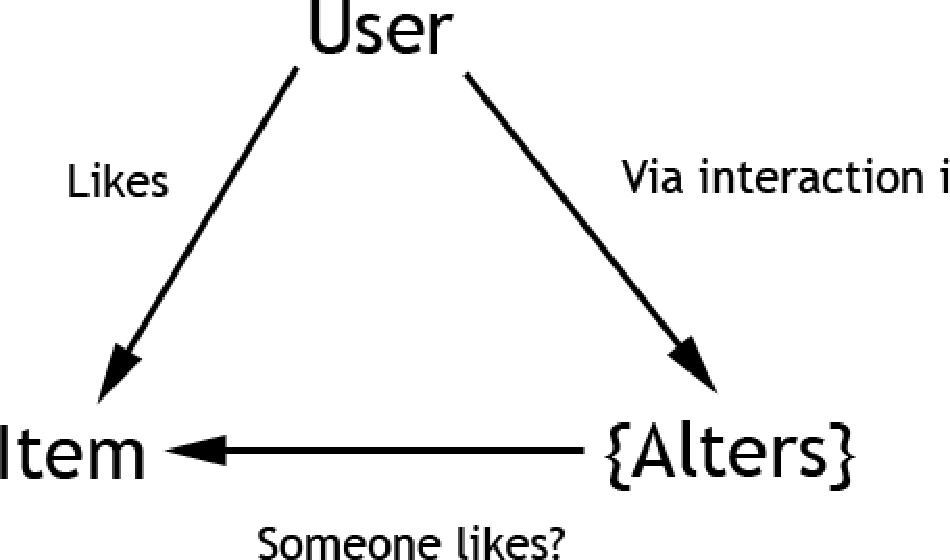
\includegraphics[scale=0.5]{imgs/alters.pdf}
		\caption{Alters paradigm. A user $u$ likes some item $v$, a $Relationship_{u,z}$ is defined via some affinity $i$ (in this example we use \emph{interactions}) uniquely defined
		for each affinity feature, to create our set of $alters_{u,v,i}$.}
	\end{center}
\end{figure}

\item  Exposure of a user $u$
to an item $v$ is the number of friends of $u$ who have liked $v$. An exposure limit where $Exposure_{u,v} = \displaystyle\sum_{z}^{N} (Friend_{u,z} \wedge Liked_{z,v})$ where this exposure can be 
limited by some $k$ with the condition $Exposure_{u,v} >= k$. Thus ensuring some $k$ number of friends have liked a link $v$.

This exposure can be visualised in the figure below:

\begin{figure}[h!]
	\begin{center}
		\includegraphics[scale=0.5]{results/imageLiked.png}
		\caption{Here we see an example of a link $v$ posted to a friends wall, which has subsequently been liked by two friends $z$. This 
				 demonstrates an exposure of $2$ for item $v$.}
	\end{center}
\end{figure}

\item A data-set $D$ comprised of $D = \{(u,v,x) \to y\}$ where $u \in U$, $v \in V$ and the binary response $y \in \{0,1\}$ 
where $0$ represents a dislike and $1$ represents a like. 
\end{itemize}

\section{Affinity Features}
\label{sec:features}

Given the vast amount of potential information available about users on Facebook, we need to break this information down into individual 
features.The two distinct categories we will group these features under are \emph{user interactions} and \emph{user preferences}. 
\emph{User interactions} involve explicit affinity relationships between users, while \emph{user preferences} involve latent 
similarities expressed between users.

The individual components of these affinity based categories are displayed below:

\emph{User interactions}:
\begin{itemize}
\item \textbf{Interactions} : Posts, tags, likes, comments between users.
\item \textbf{Outgoing Messages} : Messages sent to other users.
\item \textbf{Incoming Messages} : Messages received from other users.
\end{itemize}

\emph{User preferences}:
\begin{itemize}
\item \textbf{Demographics} : Age, gender and location of a user.
\item \textbf{Favourites} : A users favourite preferences for activities, books, athletes, teams, movies, music, sports, television, people and interests.
\item \textbf{Groups} : All groups a user has joined.
\item \textbf{Pages} :  All pages a user has liked.
\end{itemize}

Each of these affinity features will be used individually to train and test our classifiers defined below and are discussed 
in explicit detail under their separate sections of this thesis.
During our analysis we will compare the predictiveness of each of these affinity features individually and in combination.
Each feature will also be tested against some exposure to analyse the differences in results.

\section{Previous Work}
\label{sec:pw}

Two general approaches to prediction in a social context are \emph{content-based filtering} (CBF) \cite{newsweeder} which exploits 
item features based on items a user has previously liked and  \emph{collaborative filtering} (CF) 
\cite{collab_filtering} which exploits the current users preferences as well as those of other users. 

Previous work defined the term \emph{social} CF (SCF) \cite{joseph} which augments traditional CF methods with additional social 
network information, the results of this previous work and analysis using live user trials came to the conclusion that the approach of SMB
provided the best results for this data set and as such will be used as a baseline.

These methods of CBF, CF and SCF result in a user gaining some similarity measure between other users, while the affinity features we 
explore during this thesis are based on explicit individual \emph{user interaction} and \emph{user preference} features and result in different 
models and predictions based on our feature selection.

\section{Training and Testing}
\label{sec:tt}

All evaluation is applied using $10$ fold cross validation wherein the data is partitioned into $10$ complementary subsets, 
eight folds ($80\%$ of data) for training and two folds ($20\%$ of data) for testing.

The training and testing process is repeated $10$ times for each set of fold data. These results are then averaged to produce our 
estimates and standard error. The benefit of this method over repeated sub-sampling is all data points are used for both training 
and validation.

\section{Recommendation Algorithms and Baselines}
\label{sec:meth}

Each classification algorithm is passed the training data for each fold as outlined above. The classifier 
builds a model representation of the data and applies this model to the test set to classify each test item into either a dislike $0$ or 
a like $1$.

All affinity feature analysis carried out in this thesis will be performed on the following classification algorithms:

\subsection{Constant}
\label{sec:const}

The constant predictor returns a constant result irrespective of the affinity feature selected. Namely, this predictor returns dislike
regardless of the affinity feature represented by $X$. The most common result in our data set is dislike and hence this dislike 
predictor is displayed in all comparison analysis, tables and graphs.

\subsection{Social Match Box}
\label{sec:sr}

SMB is an extension of existing SCF techniques~\cite{lla,socinf} which constrain the latent space to enforce users 
who have similar preferences to maintain similar latent representations when they interact heavily.

SMB uses the social regularization method which incorporates user features to learn
similarities between users in the latent space which allows us to incorporate the social information of the Facebook data ~\cite{joseph}.

This objective component constrains users with a high similarity rating to have the same values in the latent feature space, which
models the assumption that users who are similar socially should also have similar preferences for items.

\subsection{Naive Bayes}
\label{sec:nb}

NB is a basic probabilistic classifier which involves applying Bayes' theorem using strong conditional independence 
assumptions between each feature in $X$. During training each element $i$ in $X$ is devised to contribute some 
evidence that this $x_i$ belongs to either a like or dislike classification, during testing the class with the highest probability 
when applied to the model is the classification predicted. 

With feature vector $f \in \mathbb{R}^F$ derived from $(x,y) \in D$, denoted as $f_{x,y}$. NB learns a conditional model of the form 
$p(C|F_1, \dots, F_n)$ over a dependent class variable $C$ conditioned on the feature variables $F_1, \dots, F_n$. Applying both Bayes' rule 
and conditional independence assumptions the model can be rewritten as $p(C|F_1, \dots, F_n) = p(C) \displaystyle\prod_{i=1}^n p(F_i|C)$.

Classification of our test vector is achieved by choosing the most probable class of either like ($1$) or dislike ($0$).
\\
$\mathrm{classify}(f_1,\dots,f_n) = \underset{c \in \{1,0\}}{\operatorname{argmax}} \ p(C=c) \displaystyle\prod_{i=1}^n p(F_i=f_i\vert C=c)$.

\subsection{Logistic Regression}
\label{sec:lr}

LR directly estimates parameters based on the training data assuming a parametric form of the distribution.
LR predicts the odds of a feature vector $X$ being either a like or a dislike by converting a dependent variable and 
one or more continuous independent variable(s) into probability odds.

The probability $p_i$ is modelled using a linear predictor function $l(i)$, the linear predictor function of a particular point $d$ 
is written as $l(i) = \beta_0 + \beta_1 x_{1,i} + \cdots + \beta_M x_{m,i}$, where each data point $d$ is associated with an explanatory 
feature vector $X$ and $\beta_0, \ldots, \beta_M$ are regression co-efficients indicating the relative effect of a particular 
explanatory variable $x_{m,i}$ on the prediction.

The probability of a particular outcome is linked to the linear prediction function, 
$\operatorname{logit}(\mathbb{E}[Y_i|x_{1,i},\ldots,x_{m,i}]) = \operatorname{logit}(p_i)=\ln\left(\frac{p_i}{1-p_i}\right) = \beta_0 + \beta_1 x_{1,i} + \cdots + \beta_M x_{m,i}$
Where the class of either dislike ($0$) or like ($1$) with the higher probability is the prediction made.

The LR implementation used during this thesis is \emph{LingPipe} \cite{lin}.

\subsection{Support Vector Machine}
\label{sec:svm}

SVM is a supervised learning machine based on a set of basis functions which help construct 
a separating hyperplane between data points. Training involves building the relevant hyperplanes which can then be used for testing. 
Each data point is classified as a like or dislike depending on which side of the hyperplane it falls.

With feature vector $f \in \mathbb{R}^F$ derived from $(x,y) \in D$, denoted as $f_{x,y}$. A linear SVM learns a weight vector $w \in \mathbb{R}^F$
such that $w^T f_{x,y} > 0$ indicates a like classification of $f_{x,y}$ and $w^T f_{x,y} \leq 0$ indicates a dislike classification.

The SVM implementation used during this thesis is \emph{SVMLibLinear} \cite{cjlin}.

\section{Evaluation Metrics}
\label{sec:notation}

When evaluating the success of each affinity feature at correctly classifying an item, the following metrics are used:

\begin{itemize}
\item A \emph{true positive} (TP) prediction refers to when the prediction correctly identifies the class as true. 
\item A \emph{false positive} (FP) occurs when the prediction is true, but the true class was false.
\item A \emph{false negative} (FN) occurs when the prediction is false but the actual class is true.
\end{itemize}

These definitions can be visualised using the table below:

\begin{table}[tbh!]
\centering
\begin{tabular}{r|l|l|l|}
\multicolumn{1}{r}{}
 &  \multicolumn{3}{c}{$y$} \\
 \cline{2-4}
& & \textbf{T} & \textbf{F} \\ 
\cline{2-4}
$\hat{y}$ & \textbf{T} & TP & FP \\
\cline{2-4}
& \textbf{F} & FN & TN \\
\cline{2-4}
\end{tabular}
\caption{Actual and prediction comparison table.}
	\label{tab:revpol}
\end{table}

Where $y$ represents the true class value $y \in \{0,1\} : actual$ and $\hat{y}$ represents the class prediction $\hat{y} \in \{0,1\} : prediction$.

Accuracy relates to the closeness to the true value. In the context of our results, the accuracy refers to the number of correct classifications 
divided by the size of the data set.

\[ \text{accuracy} = \frac{\text{number of correct classifications}}{\text{size of the test data set}}\]

Precision relates to the number of retrieved predictions which are relevant. In the context of our results, the precision refers to the number of TP predictions 
divided by the sum of the TP and FP predictions.

\[ \text{precision} = \frac{\text{number of TP}}{\text{number of TP + number of FP}}\]

Recall refers to the number of relevant predictions that are retrieved. In the context of our results, recall refers to the number of TP predictions 
divided by the sum of the TP and FN predictions.

\[ \text{recall} = \frac{\text{number of TP}}{\text{number of TP + number of FN}}\]

The f-score combines and balances both precision and recall and is interpreted as the weighted average of both precision and recall. 

\[ \text{f-score} = 2 \times \frac{\text{precision} \times \text{recall}}{\text{precision} + \text{recall}}\]

The main metric we use for analysis, tabulation and graphing in our results is accuracy.

%%% Local Variables: 
%%% mode: latex
%%% TeX-master: "thesis"
%%% End: 
